\documentclass{ohm_project_description}
\usepackage[english]{babel}

\projecttitle{Drone Light Painting – Coordinated Light Image Generation with Micro-Drones}
\projectauthor{Mobile Robotics Lab}
\projectdate{2026}

\begin{document}

\maketitle
\thispagestyle{fancy}

\vspace*{-2.5cm}
\begin{figure}[h!]
    \centering
    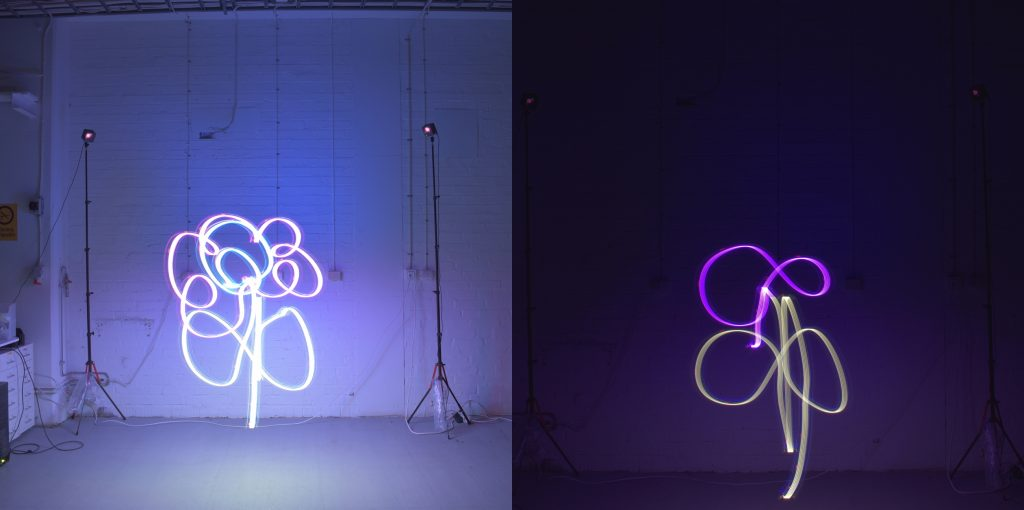
\includegraphics[height=4cm]{img/lightpainting.png}
\end{figure}

A group of Crazyflie micro-drones is now available at the AerodrOHM and can be programmed for coordinated formation flights. The goal of this thesis is to implement a demonstration in the style of drone light painting: the drones execute predefined flight patterns to generate spatial light images that can be captured photographically using long-exposure photography. The Bitcraze Lighthouse Painting project serves as thematic orientation.

Suitable flight paths are to be designed, covering both simple geometric shapes and more complex patterns such as lettering or logos. The trajectories must be planned so that collisions between drones are reliably avoided and temporal synchronisation is ensured, accounting for the limited flight time of the micro-drones. Building on trajectory planning, the coordinated control of multiple drones in the swarm is to be realised. Practical testing takes place in the AerodrOHM flight space, where the resulting light images will be photographically documented.

\section*{Work Packages}
\begin{itemize}[leftmargin=0.5cm]
    \setlength\itemsep{.1em}
    \item Familiarisation with the drone platform and its programming interface
    \item Design and implementation of flight paths for various light patterns
    \item Coordination and synchronisation of multiple drones in the swarm
    \item Experimental testing and photographic documentation of the light images
\end{itemize}

\section*{Requirements}
\begin{itemize}[leftmargin=0.5cm]
    \setlength\itemsep{.1em}
    \item Good programming skills in Python
    \item Interest in autonomous flight and multi-robot systems
    \item Basic understanding of coordinate systems and spatial geometry
\end{itemize}

\vspace{0.5cm}
This topic can be completed as a \textbf{project, bachelor's or master's thesis} subject to agreement.

\vfill
\textcolor{ohm_red}{\rule{\linewidth}{0.4mm}}
\textbf{\textcolor{ohm_red}{Mobile Robotics Lab}} \\
\begin{tabular}{@{}ll}
\textbf{Supervisor:} & Prof. Dr. Christian Pfitzner \\
\textbf{E-Mail:}     & \href{mailto:christian.pfitzner@th-nuernberg.de}{christian.pfitzner@th-nuernberg.de} \\
\end{tabular}

\end{document}
